\documentclass[11pt]{amsart}
\usepackage{graphicx,xspace}
\usepackage{fullpage}
\usepackage{hyperref}
\usepackage{amsmath}
\usepackage{amsfonts}
\usepackage{verbatim}

\newenvironment{definition}[1][Definition]{\begin{trivlist}
\item[\hskip \labelsep {\bfseries #1}]}{\end{trivlist}}
\newenvironment{example}[1][Example]{\begin{trivlist}
\item[\hskip \labelsep {\bfseries #1}]}{\end{trivlist}}



\title{ADAM: Analysis of Discrete Models of Biological 
Systems Using Computer Algebra} 
\author{Franziska Hinkelmann$^{a,b}$, 
Madison Brandon$^{c,*}$,
Bonny Guang$^{d,*}$,
Rustin McNeill$^{e,*}$, \\
Grigoriy Blekherman$^{a}$, 
Alan Veliz-Cuba$^{a,b}$, 
Reinhard Laubenbacher$^{a,b}$}

\begin{document}
\maketitle
{\footnotesize
     \centerline{$^a$Virginia Bioinformatics Institute, Blacksburg, VA 24061-0123, USA} 
}

{\footnotesize
     \centerline{$^b$Department of Mathematics,
      Virginia Polytechnic Institute and State University, Blacksburg, VA 24061-0123, USA} 
}

{\footnotesize
     \centerline{$^c$University of Tennessee - Knoxville, Knoxville, TN 37996-2513, USA} 
}

{\footnotesize
     \centerline{$^d$Harvey Mudd College, Claremont, CA 91711-5901, USA} 
}


{\footnotesize
     \centerline{$^e$University of North Carolina - Greensboro, Greensboro, NC 27402-6170, USA} 
}

{\footnotesize
     \centerline{$^*$These authors contributed equally} 
}

%%%%%%%%%%%%%%%%%%%%%%%%%%%%%%%%%%%%%%%%%%%%%%%%%%%%%%%%%%%%%%%%%%
% should we remove all we/our from the abstract? F
% proteins or genes 
\begin{abstract}
Many biological systems are modeled qualitatively with discrete models, such as 
probabilistic Boolean networks, logical models, bounded petri-nets, and agent-based models.
Simulation is a common practice for analyzing discrete models, but many systems are far too large
to capture all the relevant dynamical features through simulation alone. We convert discrete models into algebraic models
and apply tools from computational algebra to analyze the dynamics of discrete systems. 
The key feature of biological systems that is exploited by our algorithms is their sparsity: while the number of genes (or agents) in a
biological network may be quite large, each gene is affected only by a small number of other genes. This allows for fast Gr\"{o}bner basis 
computations in the algebraic models, and thus efficient analysis.
All algorithms and methods are available in our package Analysis of Dynamic
Algebraic Models (ADAM), a `modeler friendly' web-interface
that allows for fast analysis of large models, without requiring understanding of the underlying mathematics or any software installation.
\end{abstract}


%%%%%%%%%%%%%%%%%%%%%%%%%%%%%%%%%%%%%%%%%%%%%%%%%%%%%%%%%%%%%%%%%%
\section{Background} % or Introduction? F

\begin{comment}
% Modeling, Discrete vs continuous models
Mathematical modeling is a crucial tool in understanding the dynamic behavior of
biological systems. Continuous differential equations models are commonly used, but they rely on
the knowledge or estimation of parameter rates, which are often hard to obtain. Discrete models
offer slightly coarser qualitative information, but do not require the fine parameter data to set up.
In many instances the qualitative is already quite interesting and unknown. 
%Discrete models are often very intuitive and easily understood by life
%scientists.
\end{comment}
% Different discrete models and lack of analysis tools
Discrete models are widely used in studying dynamical behavior of biological systems. Model types include
(probabilistic) Boolean networks, logical networks, Petri-nets, Cellular
automata, and Agent-based (individual-based) models. 
However, there is a lack of tools
for analyzing dynamical behavior of large-scale discrete models. Commonly, the analysis is performed by simulation, meaning that an
initial configuration of the system is iterated a prescribed number of times, or until a
steady state is found. Since the number of initial configurations grows exponentially in the number of variables, simulation
will not provide a complete picture of dynamical behavior for large models.
Simulation is especially inefficient for non-deterministic
systems, since simulations must be run many times to obtain meaningful
probability estimates.

% Math framework and Groebner basis
All of the different types of discrete models mentioned above can be
converted into the unified framework of polynomial dynamical systems
\cite{Alan:Bioinf2010, Hinkelmann:2010}. This allows us to apply tools from
computational commutative algebra to analyze their dynamics. 

%%%%%%%%%%%%%%%%%%
\section{Results}
% ADAM available for free, platform independent
We developed an
online software package ADAM, Analysis of Dynamic Algebraic Models \cite{ADAM}, which automatically converts discrete models into polynomial dynamical
systems, and then analyzes their dynamics by using various computational algebra techniques. Even for large systems, ADAM
computes key dynamic features, such as fixed points, in a matter of seconds.
ADAM is available online free of charge. It is platform
independent and does not require installation of any software or computer
algebra tool. 
%% different input types
ADAM supports the following {\bf inputs}.
\begin{itemize}
  \item Logical models generated with GINsim \cite{GINsim}
  \item Petri-nets generated with Snoopy \cite{Snoopy}
  \item polynomial dynamical systems
  \item Boolean networks
  \item probabilistic polynomial dynamical systems \cite{shmulevich}.
\end{itemize}
Logical models, Petri-nets, and Boolean networks are automatically converted
into the corresponding polynomial dynamical system as described in
\cite{Alan:Bioinf2010}, so that algorithms from computational
algebra can be used to analyze the dynamics. 

% output
We developed and implemented several different algorithms that allow one to analyze 
important features of algebraic models when they are too large for pure simulation. 
Most algorithms rely on Gr\"obner basis calculations to find key dynamic
features. 
Since the polynomials in the algebraic
models originate from biological systems, we can exploit their structural
features to secure very fast Gr\"obner basis computations. 
For small enough models, ADAM generates a graph of the complete phase space.
When the phase space is too large to be drawn or when a visualization is not
needed, ADAM generates the following {\bf output}.
\begin{itemize}
  \item a graph of wiring diagram
  \item fixed points (for deterministic and probabilistic systems)
  \item limit cycles of length $m$
  \item trajectories originating from a given initial state until a stable
  attractor is found
  \item dynamics for synchronous or asynchronous updates
  \item functional circuits for Boolean networks
  \item a complete description of the phase space for conjunctive/disjunctive
  networks.
\end{itemize}

%explain that everything is a polynomial and how equations relate to dynamics
The key idea behind our algorithms is that discrete models have finitely many states and computations 
can be performed over a finite field \cite{Alan:Bioinf2010,
Hinkelmann:2010}. Since any function over a finite field is a polynomial
\cite{Lidl:1997} we convert discrete models into polynomial dynamical systems
and use commutative algebra algorithms. More specifically, the problem of finding fixed points and limit cycles
can now be reformulated as solving a system of polynomial equations. We use Gr\"{o}bner basis techniques to solve the 
resulting system of polynomial equations. Gr\"obner basis calculation is for polynomial systems what
Gauss-Jordan elimination is for linear systems: a structured way to transform
the original system to triangular shape without changing its solution space.
The triangular shape of the resulting systems allows for stepwise retrieval of the solutions of the system.

% Sparse systems
The efficiency of the Gr\"obner basis calculations is largely dependent on the
assumption that most discrete models arising from biological systems are
sparse, meaning that every variable is only affected by a small subset of the
total variables in the system. It has been suggested, that in robust gene
regulatory networks genes are regulated by only a handful of regulators
\cite{Leclerc:2008}. Thus the PDSs representing such biological networks are
sparse, i.e., each function depends only on a small subset of the total nodes.

% heuristic explanation for why we think the GB algorithm is fast on
%sparse systems..
In the worst case, computing Gr\"obner bases for a set of polynomials has a
complexity of doubly exponential in the number of solutions to the system.
However, in practice, Gr\"{o}bner bases are computable in a reasonable time, and
for the sparse systems over a finite field that are common in discrete
biological models, it is actually fairly fast. 
%In the first place, computing
%Gr\"{o}bner bases in modular form have been shown to be much faster usually
%\cite{Brown:1971}. 
Working with sparse polynomials means that simpler
S-polynomials, usually of short length, will be added, causing the Groebner
basis computation to be easier.
Based on benchmarking tests for 
25 logical models of biological systems \cite{GINsim} 
and randomly generated systems,
the computations are very fast, and finish on the scale of
seconds.

\section{Application} \label{benchmarks}
% Example application
We demonstrate the power of ADAM on a well understood model of the expression
pattern of the segment polarity genes in Drosophila melanogaster.  The Boolean
model presented in \cite{AO} consists of 60 variables, resulting in a phase
space with over $10^{18}$ states. ADAM correctly identifies the fixed points
in less than one second. In addition, ADAM computes that are there no limit
cycles of length two or three. The model has not been analyzed previously for
limit cycles. The absence of two- and three cycles strengthens confidence in
the model, since oscillatory behavior has not been observed experimentally.
The model file in ADAM format can be accessed at \cite{DrosophilaModel}. 

We analyzed logical models
available in the GINsim model repository \cite{GINsimRepo} as of August 2010. The
repository consists of models in GINsim XML format previously published in
peer reviewed journals. We converted all but two models into polynomial
dynamics systems. For these 27 models we computed the fixed points. Almost all
calculations finished in less than a second. The two largest networks,
consisting of over $10^{30}$ states, took around 20 minutes each, see 
Figure \ref{fig:chart}. 

In addition to the published models in \cite{GINsimRepo}, we analyzed 
randomly generated networks
that have the same sparse structure that we
expect from biological systems. We tested a total of 50 networks with
50-100 nodes ($10^{15} - 10^{30}$ states) and up to 2 inputs per variables. The 
fixed point calculations took less than half a second for each network on
a 2.7 GHz computer. 


%\begin{table}[h]
%	\centering
%	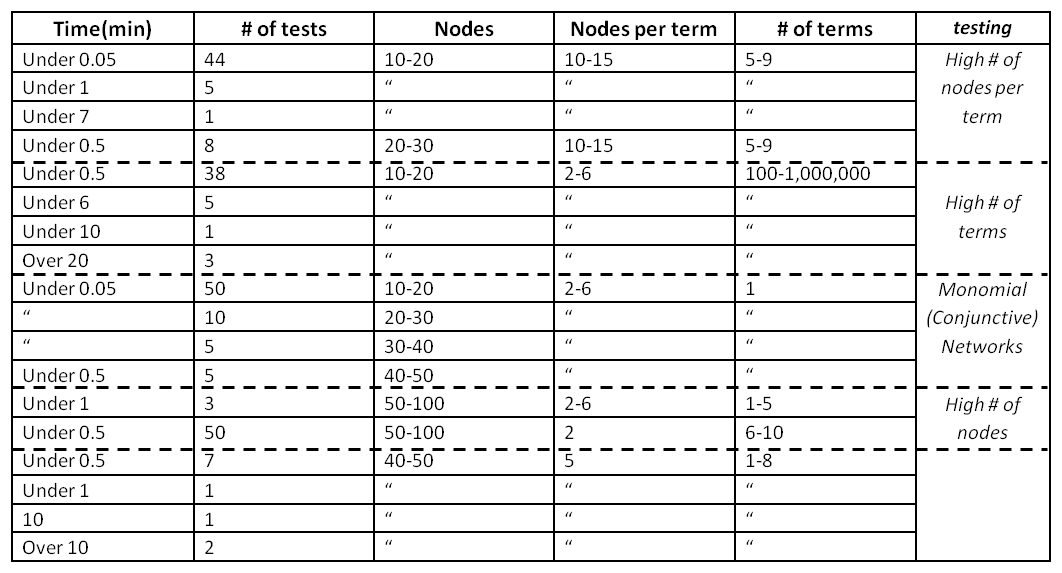
\includegraphics[scale=0.8]{benchmarkTable.png}
%	\caption{Results of benchmark tests for randomly generated networks}
%	\label{tab:GBbenchmarks}
%\end{table}
\begin{figure}[htb]
  \centering
  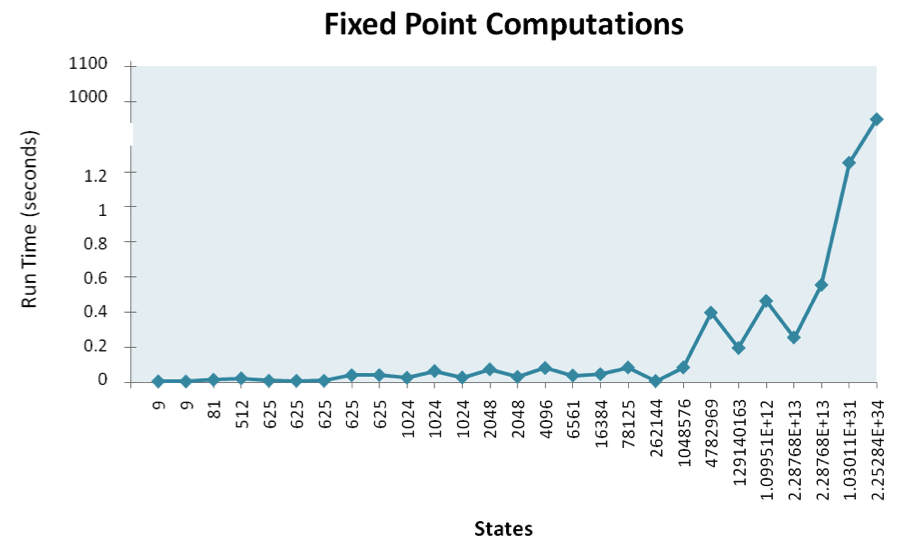
\includegraphics[width=0.95\textwidth]{GINSimChart.png}
  \caption{Runtime of fixed points calculations of several logical models from
  \cite{GINsimRepo}. Executed on a 2.7 GHz computer.}
  \label{fig:chart}
\end{figure}

%%%%%%%%%%%%%%%%%%%%%%%%%%%%%%%%%%%%%%%%%%%%%%%%%%%%%%%%%%%%%%%%%%
\section{Methods}
\subsection{Polynomial Dynamical Systems}
To be self-contained, we briefly explain PDS and their key features. 
Several types of discrete models, including Logical models, Petri
Nets, and Agent-Based models, can be translated into PDS \cite{Alan:Bioinf2010,Hinkelmann:2010}.

\subsubsection{Polynomial Dynamical System (PDS)}
A {\bf polynomial dynamical system} \cite{JLSS} over a finite field $k$ is a function
$$f = (f_1, \ldots, f_n) : k^n \rightarrow k^n,$$ 
with coordinate functions $f_i \in k[x_1, \ldots , x_n]$. Iteration of $f$ results
in a time-discrete dynamical system. PDSs are special cases of finite
dynamical systems, which are maps $X^n \rightarrow   X^n$ over arbitrary
finite sets $X$.

PDS have several dynamic features of biological
relevance. These include the number of components, component sizes, fixed
points, limit cycles, and limit cycle lengths. 
\begin{example}
Let $k= \mathbb F_2$ and $f = (f_1, f_2, f_3) : \mathbb F_2^3 \rightarrow
\mathbb F_2^3$ with 
\begin{align*}
f_1 &= x_1x_2x_3+x_1x_2+x_2x_3+x_2 \\
f_2 &= x_1x_2x_3+x_1x_2+x_1x_3+x_1+x_2 \\
f_3 &= x_1x_2x_3+x_1x_3+x_2x_3+x_1+x_2.
\end{align*}
The wiring diagram of $f$, which shows the static interaction of the three
variables, is
depicted in Figure \ref{fig:ex} (left) along with its phase space in Figure
~\ref{fig:ex} (right).
The phase space shows the temporal evolution of the systems. Each state is 
represented as a vector of the values of the three variables $(x_1, x_2,
x_3)$. 
The PDS described by $f$ has
two stable attractors: a fixed points, $(000)$, and a limit cycle of length
three, consisting of the states $(010)$, $(111)$, and $(011)$.
\end{example}

\begin{figure}[ht]
  \centering
  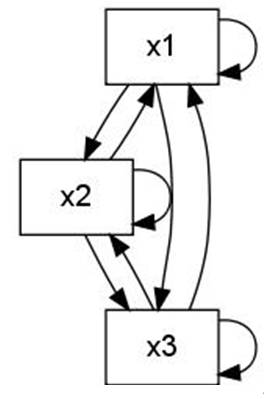
\includegraphics[scale=0.55]{exampleWD.jpg}
  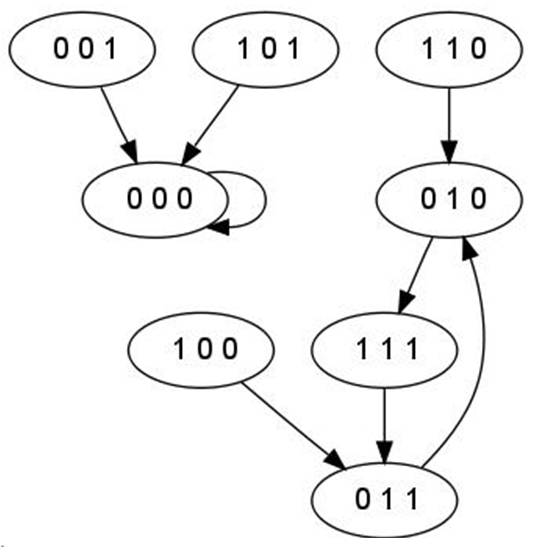
\includegraphics[scale=0.55]{exampleSS.jpg}
  \caption{(left) 
  Wiring diagram: static relationship between variables
  (right)
  Phase space: temporal evolution of the system
  }
  \label{fig:ex}
\end{figure}

\subsubsection{Probabilistic Polynomial Dynamical System}
A {\bf probabilistic PDS} over a finite field $k$ is a collection of functions
$$f = (\{f_{1,1}, \ldots, f_{1, r_1}\}, \ldots, \{f_{n, 1}, \ldots, f_{n, r_n}
\}) : k^n \rightarrow k^n,$$ 
together with a probability distribution for every coordinate that assigns the
probability that a specific function is chosen to update that coordinate. 
The coordinate functions $f_{i,j}$ are in $k[x_1, \ldots , x_n]$. 
Probabilistic PDS, specifically Boolean probabilistic networks (PBN), have been studied
extensively in \cite{shmulevich}. 

ADAM analyzes probabilistic PDS. It can simulate the
complete phase space for small enough models, by generating every possible
transition and labeling the edge with its probability according to the
distribution. If no distribution is given, ADAM assumes a uniform distribution
on all functions. For large networks, ADAM's {\it Algorithm} choice computes
fixed points of probabilistic networks.


%%%%%%%%%%%
\subsubsection{Functional Edges}
An edge in the wiring diagram from $x_i$ to $x_j$ is considered
functional, if there exists a state $\hat x = (\hat x_1,  \ldots, \hat x_n)$ such
that $f_j( \hat x_1,  \ldots, a, \ldots \hat x_n) \neq f_j(\hat x_1, \ldots, b, \ldots
\hat x_n)$, where $a$ and $b$ are values for $x_i$, in other words, if there
is at least one state, such that changing only $x_i$ but keeping all other
values fixed, changes the next state of $x_j$. 
In ADAM, all edges in the wiring diagram are functional. 

For Boolean networks, ADAM identifies all functional circuits. A circuit is a
closed directed path in the wiring diagram and it is functional, if all its
edges are functional. For further discussion of
functional circuits, see \cite{Chaouiya}. 

%%%%%%%%%%%%%%%%%%%%%%%%%%%%%%%%%%%%%%%%%%%%%%%%%%%%%%%%%%%%%%%%%%
\section{Algorithms}
\subsection{Analysis of stable attractors}
Every attractor in a PDS is either a
fixed point or a limit cycle. For small models, ADAM determines the complete
phase space by enumeration, for large models, ADAM computes fixed points and
limit cycles of a given length. 

A state is a fixed point, if it transitions to itself after one update of the
system. A state is part of a limit cycle of length $m$, if,
after $m$ updates, it results in itself. Any fixed points of a PDS satisfies
the equation $f(x) = x$, as no coordinate of $x$ is changing as it is updated. 
Similarly, states of a
limit cycle of length $m$ satisfy the equation $f^m(x) = x$. ADAM computes all
fixed points by solving the system $f_i(x) - x_i = 0$ for $i \in \{1, \ldots,
n\}$ simultaneously. To efficiently solve the resulting systems of polynomial
equations, we first compute the Gr\"obner
basis in lexicographic order for the ideal generated by the equations.
By the elimination and extension theorem \cite{IVA}, choosing a lexicographic order
allows to easily obtain the solutions.
We use the Gr\"obner basis calculations distributed with Macaulay2 \cite{Macaulay2}, a
computer algebra system, and found that for quotient rings over a finite field
the implementation `Sugarless' is more efficient than the default algorithm
with `Sugar' \cite{Sugar:1991}. 
For limit cycles of length $m$, the solutions of $f^m(x)=x$ are found and then
grouped into cycles, by applying $f$ to each of the solutions. 

%%%%%%%%%%%
\subsection{Conjunctive/Disjunctive Networks}
Some classes of networks have a certain structure that can be
exploited to achieve faster calculations. In \cite{conjunctive}, Jarrah et al.
show that for conjunctive (disjunctive) networks key dynamic features can be found with
almost no computational effort. Conjunctive (resp disjunctive) networks consist of
functions using only the AND (resp. OR) operator. 
We include a separate algorithm to analyze 
dynamics in the case of conjunctive/disjunctive networks as described in
\cite{conjunctive}. Currently,
this option only works on strongly connected graphs


%%%%%%%%%%%%%%%%%%%%%%%%%%%%%%%%%%%%%%%%%%%%%%%%%%%%%%%%%%%%%%%%%%
\section{Conclusion}
Discrete Modeling techniques are a useful tool for analyzing biological
systems. Upon translating a discrete model, such as logical networks,
petri-nets, or agent-based models into an algebraic model, rich mathematical
theory becomes available. This enables one to
avoid simulation which is limited because of combinatorial explosion. The algorithms 
we developed are fast for sparse systems, a structure maintained by most biological
systems. All algorithms have been included in the software package ADAM\cite{ADAM}, 
which is user-friendly and available as a free web service. 
ADAM is highly suitable to be used in a class room as a first
introduction to discrete models as it does not require the students to run
anything else but a web browser.
We hope to expand ADAM to an all-encompassing Discrete Toolkit which incorporates more 
analytical methods, better visualization, and automatic conversion for more model types. 
We also hope to analyze controlled algebraic models and expand theory to stochastic systems. 

%%%%%%%%%%%%%%%%%%%%%%%%%%%%%%%%%%%%%%%%%%%%%%%%%%%%%%%%%%%%%%%%%%
\section*{Acknowledgments}
The authors would like to thank Prof Monika Heiner for clarifying the Petri
net terminology.
Funding: REU NSF Fund number 0755322, Army research grant, Alan's
NSF fund, other funds?
\bibliographystyle{plain}
%\bibliographystyle{authordate1}
\bibliography{ADAM}
\end{document}
